\documentclass[journal]{IEEEtran}

% Additional packages
\usepackage{graphicx}
\usepackage{amsmath}
\usepackage{lipsum}
\usepackage{hyperref} 
\usepackage{qrcode}
\usepackage{float}
\usepackage{subcaption}

\begin{document}

\title{Determination of Resistance Using Wheatstone Bridge Method}
\author{YOUR NAME\\
ISTANBUL UNIVERSITY FACULTY OF SCIENCE\\
DEPARTMENT OF PHYSICS\\
Instructor: INSTRUCTOR NAME\\
Experiment Date: DD.MM.YYYY , Report Submission Date: DD.MM.YYYY\\
Course \& Section Number: PHYS2305}

\maketitle

\begin{abstract}
    This experiment investigates the resistance measurement of an unknown resistor using the Wheatstone Bridge method and the determination of resistivity based on conductor dimensions. The relationship between resistivity, conductor length, and cross-sectional area is explored. Calculations of resistances, based on various lengths and diameters, verify the theoretical expectations, supporting the use of the Wheatstone Bridge for accurate resistance determination. Results are cross-verified with a hand-drawn graph on millimetric paper.
\end{abstract}
    

\section{Introduction}
The purpose of this experiment is to measure an unknown resistance using the Wheatstone Bridge and to determine the resistivity based on conductor dimensions. The Wheatstone Bridge is widely used for precise resistance measurements and operates on a balance of voltage in a four-resistor network. Additionally, by measuring resistance and wire dimensions, we can calculate the resistivity, an intrinsic property that affects a material's conductive behavior. Understanding resistivity is essential in material science and circuit design, where it directly impacts current flow and energy efficiency.
\section{Theory}
Ohm’s Law describes the fundamental relationship between current, voltage, and resistance in a conductor, expressed mathematically as:
\begin{equation}
    R = \frac{V}{I}
    \label{eq:ohmslaw}
\end{equation}
where \( R \) is the resistance in ohms, \( V \) is the voltage in volts, and \( I \) is the current in amperes. This law forms the basis for understanding how resistances behave in an electrical circuit.

In a Wheatstone Bridge configuration, four resistors are arranged in a diamond shape. When the bridge reaches equilibrium—meaning there is no current flowing through the galvanometer connected between the midpoints of two branches—the ratio of the resistances can be expressed as:
\begin{equation}
    \frac{R_1}{R_2} = \frac{R_3}{R_4}
    \label{eq:wheatstone}
\end{equation}
This equation arises from the principle of balance in the bridge, where the potential difference across the galvanometer is zero. The balance condition allows us to determine an unknown resistance \( R_1 \) by using known resistances \( R_2, R_3, \) and \( R_4 \). This relationship is fundamental for accurately measuring unknown resistances in a circuit.

Additionally, the resistivity (\(\rho\)) of a conductor, an intrinsic property based on material, relates resistance to its physical dimensions:
\begin{equation}
    R = \rho \frac{L}{A}
    \label{eq:resistivity}
\end{equation}
In this equation, \( R \) is the resistance, \( L \) is the length of the conductor, \( A \) is the cross-sectional area, and \( \rho \) is the resistivity in ohm-centimeters (\(\Omega \cdot \text{cm}\)). This formula highlights that resistance increases with length and decreases with a larger cross-sectional area.

In the context of the Wheatstone Bridge, we can also derive another important relationship. Considering the lengths of the segments of the bridge, the ratio of the unknown resistance \( R_1 \) to one of the known resistances \( R_4 \) can be expressed in terms of the lengths \( L_2 \) and \( L_3 \):
\begin{equation}
    \frac{R_1}{R_4} = \frac{L_2}{L_3}
    \label{eq:wheatstone_length}
\end{equation}
This derivation stems from the understanding that, at equilibrium, the voltage drop across \( R_1 \) is equal to the voltage drop across \( R_4 \). By knowing the lengths \( L_2 \) and \( L_3 \), we can effectively calculate the unknown resistance \( R_1 \), further reinforcing the accuracy of the Wheatstone Bridge method in resistance measurement.

The resistivity concept is vital as it affects the conductive properties of materials used in electrical circuits. Understanding the relationship between resistance, resistivity, and physical dimensions of conductors is essential for the design and analysis of electrical systems.


\section{Experimental Setup}
\label{sec:setup}
The experiment utilizes a Wheatstone Bridge setup to measure an unknown resistance. The equipment includes a galvanometer, voltage source, a known resistance box, and a variable length of resistance wire. Additionally, resistors of different values are used in various configurations to explore the Wheatstone Bridge balance condition. Figure~\ref{fig:setup} illustrates the Wheatstone Bridge configuration as referenced in the lab manual \cite{lab_manual}.

\begin{figure}[H]
    \centering
    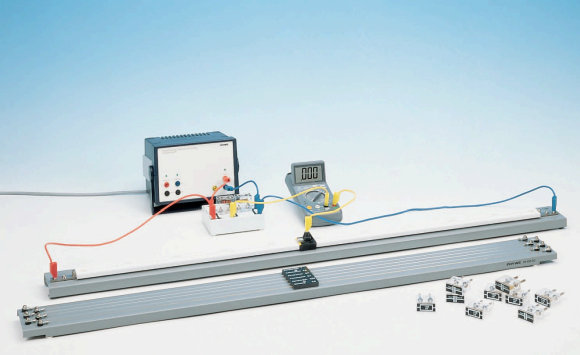
\includegraphics[width=0.45\textwidth]{IMAGES/wheatstone_bridge.png} % Replace with actual image path
    \caption{Wheatstone Bridge Experimental Setup \cite{lab_manual}.}
    \label{fig:setup}
\end{figure}

The first part of the experiment aimed to proof the relationship, $\frac{R_1}{R_4} = \frac{L_2}{L_3}$ as explained in Section~\ref{sec:procedure} 
using the setup shown in Figure~\ref{fig:known_diagram}. 

while the second part of the experiment aimed to calculate unknown resistances with different configurations 
with the help of wheatstone bridge as explained in Section~\ref{sec:procedure} 
using the setup shown in Figure~\ref{fig:unknown_diagram}. 

\begin{figure}[H]
    \centering
    \begin{minipage}{0.45\columnwidth}
        \centering
        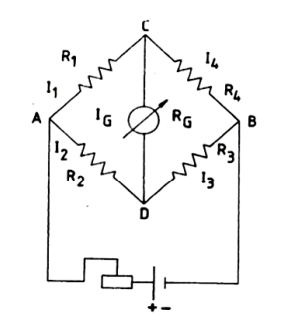
\includegraphics[width=\textwidth]{IMAGES/known_resistors_diagram.png} % Replace with actual image path
        \subcaption{Setup with known resistors to verify length-resistance relationships.}
        \label{fig:known_diagram}
    \end{minipage}
    \hfill
    \begin{minipage}{0.45\columnwidth}
        \centering
        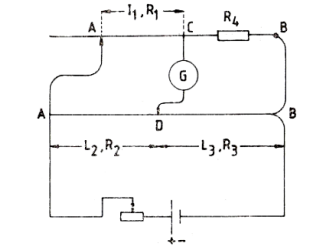
\includegraphics[width=\textwidth]{IMAGES/unknown_resistor_diagram.png} % Replace with actual image path
        \subcaption{Setup with unknown resistors for resistance calculation.}
        \label{fig:unknown_diagram}
    \end{minipage}
    \caption{Wheatstone bridge experimental setups \cite{lab_manual}.}
    \label{fig:combined_diagram}
\end{figure}





\section{Procedure}
The experiment was conducted in two stages. First, the circuit was set up as shown in Figure~\ref{fig:setup}, with known resistors in a Wheatstone Bridge configuration to verify the relationship in Eq.~\ref{eq:wheatstone_length}. Various known resistors \( R_2 \) were used, and the slider was adjusted along the resistance wire until the galvanometer indicated zero current, signaling a balanced bridge. At this point, the lengths \( L_2 \) and \( L_3 \) were recorded, and the calculated ratios were compared to verify the relationship between resistance and length.

In the second part, the setup was adjusted to include unknown resistors in place of the known resistors, as shown in Figure~\ref{fig:unknown_diagram}. The same process was followed to calculate the unknown resistance \( R_1 \), and as an example, the resistivity was specifically calculated for a wire with a diameter of 0.5 mm, using its length and measured resistance.

\label{sec:procedure}
\section{Results and Data}

\subsection{Measured Values}
Table~\ref{tab:results} presents the recorded lengths and calculated 
ratios of lengths and resistances for various configurations for known ($R_1$, $R_4$) resistances. The calculations were performed using 
the formulas derived in the previous sections, as documented in the 
\texttt{Calculations.ipynb} notebook \cite{github}.

\begin{table}[H]
\centering
\begin{tabular}{cccccc}
\hline
$R_1$ (k$\Omega$) & $R_4$ (k$\Omega$) & $L_2$ (cm) & $L_3$ (cm) & $\frac{R_1}{R_2}$ & $\frac{L_2}{L_3}$\\
\hline
4.7 & 10 & 31.6 & 68.4 & 0.47 & 0.462 \\
0.330 & 0.150 & 68.6 & 31.4 & 2.2 & 2.185\\
\hline
\end{tabular}
\caption{Measured values of resistances and lengths for verifying Eq.~\ref{eq:wheatstone_length} in the known-resistor configuration.}
\label{tab:results}
\end{table}

The purpose of Table~\ref{tab:results} is that the experimantal analysis of eq.~\ref{eq:wheatstone_length}. 

As the second part of the experiment was determination of unknown resistances 
with different diameters, experimantal data was governed and noted on Table~\ref{tab:results_part2}

\begin{table}[H]
    \centering
    \begin{tabular}{ccccc}
    \hline
    d (mm) & $L_2$ (cm) & $L_3$ (cm) & $R_1$ ($\Omega$) & $R_4$ ($\Omega$) \\
    \hline
    1 & 61.6 & 38.4 & 0.625 & 1\\
    0.7 & 43.5 & 56.5 & 1.295 & 1\\
    0.5 & 28.5 & 71.5 & 2.51 & 1\\
    0.35 & 15.8 & 84.2 & 5.32 & 1\\
    \hline
    \end{tabular}
    \caption{Measured values of lengths for calculating unknown resistances in the Wheatstone Bridge configuration.}
    \label{tab:results_part2}
\end{table}

\begin{figure}[H]
    \centering
    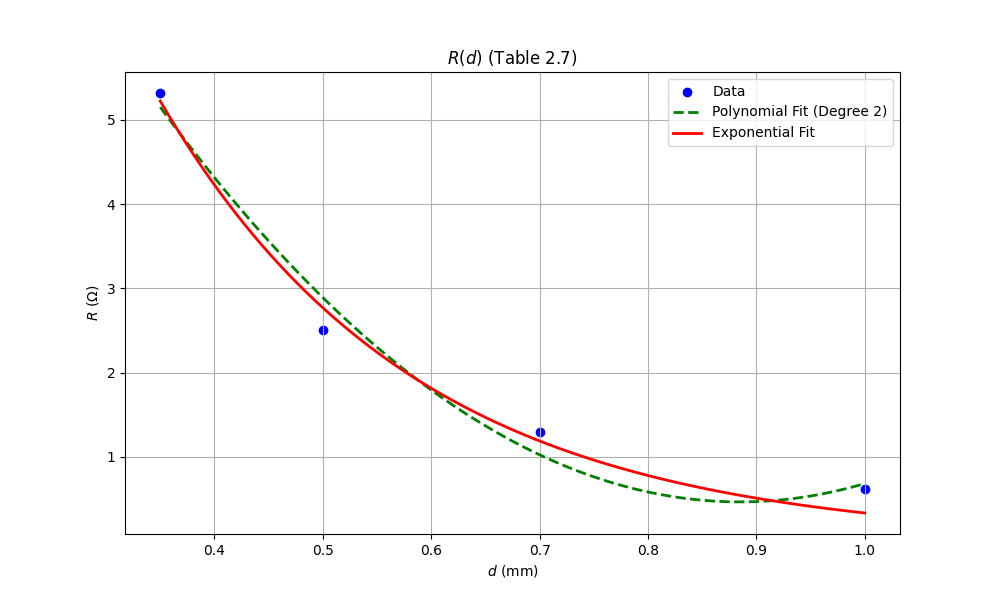
\includegraphics[width=0.5\textwidth]{output_plots/resistance_vs_diameter_table_2_7.png} % Replace with actual image path
    \caption{Plot of Resistance vs. Diameter based on experimental values \cite{lab_manual}. The graph is also hand-drawn on millimetric paper, available in the report appendix or repository \cite{graphonmillimetricpaper}.}
    \label{fig:resistance_vs_diameter}
\end{figure}

\subsection{Resistivity Calculation}
As an example, the resistivity (\(\rho\)) of a wire with a diameter of 0.5 mm was calculated using its measured resistance and length. Using the measured resistance of \( R = 2.770 \, \Omega \) for a 0.5 mm diameter wire of length \( L = 100 \, \text{cm} \), the resistivity was calculated using the following formula:
\[
\rho = \frac{R \cdot \pi \cdot \left(\frac{d}{2}\right)^2}{L}
\]
Substituting the values, the resistivity \(\rho\) was found to be approximately \(5.44 \times 10^{-5} \, \Omega \cdot \text{cm}\). This value is shown in Table~\ref{tab:resistivity}, consistent with standard resistivity values for the material used.

\begin{table}[H]
\centering
\begin{tabular}{ccc}
\hline
Diameter (mm) & Length (cm) & $\rho$ ($\Omega\cdot$cm)\\
\hline
0.5 & 100 & \(5.44 \times 10^{-5}\) \\ % Calculated resistivity value
\hline
\end{tabular}
\caption{Resistivity values for the wire with a diameter of 0.5 mm.}
\label{tab:resistivity}
\end{table}

\section{Discussion}
The Wheatstone Bridge provided accurate results, closely aligning with theoretical values. Minor discrepancies observed between calculated and expected resistances may result from several sources of error, including contact resistance in the circuit, slight inaccuracies in length measurements, or resistance fluctuations due to temperature changes in the setup. Despite these, the results for resistivity are consistent with standard values, confirming the reliability of the Wheatstone Bridge for precise resistance and resistivity measurements.

\section{Conclusion}
This experiment successfully applied the Wheatstone Bridge method to determine unknown resistance and measure resistivity. Results support the theory, showcasing the Wheatstone Bridge's precision for such measurements.


\section{Additional Resources}
For detailed information, including the Lab Manual, source code, and related experiments, visit the GitHub repository provided below or scan the QR code in 
Figure~\ref{fig:qr}.

\begin{thebibliography}{9}
\bibitem{lab_manual}
    ISTANBUL UNIVERSITY, 
    \textit{Physics Laboratory II Experiment Book: Electricity and Magnetism}, 
    Department of Physics, 2024.

\bibitem{github}
    \textit{Source code and additional experiments are available in the GitHub repository.} \\ 
    Access it at: \url{https://github.com/ibeuler/LAB-Reports}

\bibitem{graphonmillimetricpaper}
    \textit{The graph $R(d)$ fig~\ref{fig:resistance_vs_diameter} is alsow 
    drown by hand on mellimetric paper.}\\
    Available at: \url{}
    and attached to the report.
\end{thebibliography}

\begin{figure}[H]
    \centering
    \begin{minipage}{0.15\textwidth}
        \centering
        \qrcode[height=2cm]{https://github.com/ibeuler/LAB-Reports}
    \end{minipage}%
    \begin{minipage}{0.2\textwidth}
        \raggedright
        \caption{Access the GitHub repository for the lab manual, source code, and related experiments: \href{https://github.com/ibeuler/LAB-Reports}{\url{https://github.com/ibeuler/LAB-Reports}}.}
    \end{minipage}
    \label{fig:qr}
\end{figure}
\end{document}
